\section{Introduction}
The past few years have witnessed the revolution of NLP methods with 
the advent of pretrained language models~(PLMs) such as 
\textsc{BERT}~\citep{DBLP:journals/corr/abs-1810-04805} and 
\textsc{RoBERTa}~\citep{DBLP:journals/corr/abs-1907-11692}. They are first pretrained on vast amount of unlabeled text corpora using masked language modeling~(MLM) objective and 
then fine-tuned on task-specific data, offering a surge of 
improvements on a wealth of NLP tasks. However, we know very little about
\textit{what} and \textit{how much} 
knowledge embedded in PLMs actually contributes to the success. 
Notable endeavors~\citep{peters-etal-2018-dissecting,DBLP:journals/corr/abs-1901-05287,DBLP:journals/corr/abs-1905-06316} toward this understanding focus on probing linguistic knowledge therein. They demonstrated that 
pretraining did impart useful linguistic abstraction about syntax and semantics into PLMs.


More recently, several works are presenting intriguing results examining 
 relational knowledge within PLMs. Relational knowledge~\citep{speer-havasi-2012-representing,wikidata} is typically defined as describing the abstractive relationship between a pair of concepts or entities, which is crucial for facilitating language understanding.
 \citet{Petroni2020} first posed the LAMA probe, 
 an English benchmark comprising multiple sets of prompts. Each prompt is a cloze-like sentence transformed from a relational knowledge triple:
 
 \noindent
 \textbf{Knowledge Triple: }\textit{$<$bus, HasA, ?$>$} \\
 \textbf{Object Label: }seats. \\
 \textbf{Prompt: }you are likely to find \underline{~~} in a bus.

 

By substituting  \underline{~~}  with a special [MASK] token and reusing the MLM head, prompt-based relational knowledge probing provides an estimated lower bound of what PLMs know without training additional layer as in the previous linguistic probe. They showed that, even without grounded supervision, 
PLMs capture such relational knowledge at a level competitive to supervised alternatives. Subsequent works further showed that some specific prompts, acquired either through heuristical mining~\citep{DBLP:journals/corr/abs-1911-12543} or gradient-guided search~\citep{Shin2020}, can better trigger the models to correctly predict the missing object. 

Despite the mounting evidence for the existence of relational knowledge in PLMs, it remains unclear how such knowledge is represented internally. In light of this, we raise the core question in this paper:
\textit{Given a general-purpose PLM, can we disentangle it into dedicated relation-specific knowledge models?} From the perspective of representation learning, disentangled relation-specific knowledge models correspond to disentangled representation subspaces of the original language representation space. These subspaces represent knowledge inherited from different subset of MLM data expressing different relations between masked word and remaining context.


We study this question by first drawing inspiration from recent findings~\citep{DBLP:journals/corr/abs-2010-03648,DBLP:journals/corr/abs-2008-01064,inductivemlm}: \textit{the more  MLM pretraining simulates downstream task, the more successful the  transfer will be.} For example, filling \textit{like} or \textit{hate} into a cloze like ``\textit{I [MASK] this film, it's great.}'' provide a clear way in which the model can implicitly learn to perform sentiment classification. Similarly, we hypothesize that training on MLM data expressing certain relation $r$ between masked word and remaining context would lead to effective transfer on knowledge probing that targets relation $r$. 

By exploiting this correlation conversely, we offer a new way for searching disentangled representation subspaces responsible for different relational knowledge based on their transfer performance on knowledge probing task. Unlike most disentanglement learning methods that introduce parametric transformation upon original space, we restrict these subspaces to have correspondence with subnetworks of PLMs and propose an end-to-end differentiable weights pruning framework.
We show in experiment that it is possible to find subnetworks capable of representing grounded commonsense relations at non-trivial sparsity while also exhibiting evident disentanglement. \figref{fig:LAMA} exemplifies a cloze prompt where the identified subnetwork produces the valid answer \textit{seats} by attending to relevant 
context, i.e., bus,  while the original \textsc{BERT} fails. We then examine the knowledge transfer ability of these subnetworks in scenarios requiring knowledge of single or multiple commonsense relations for reasoning. Experiment on commonsense knowledge base completion show that the identified subnetworks even outperform strong supervised knowledge base completion methods. These subnetworks also outperform the original PLMs in both many-shot and zero-shot commonsense question answering tasks, when combined properly.

\begin{figure}[t]
	\centering
	\scalebox{1.0}{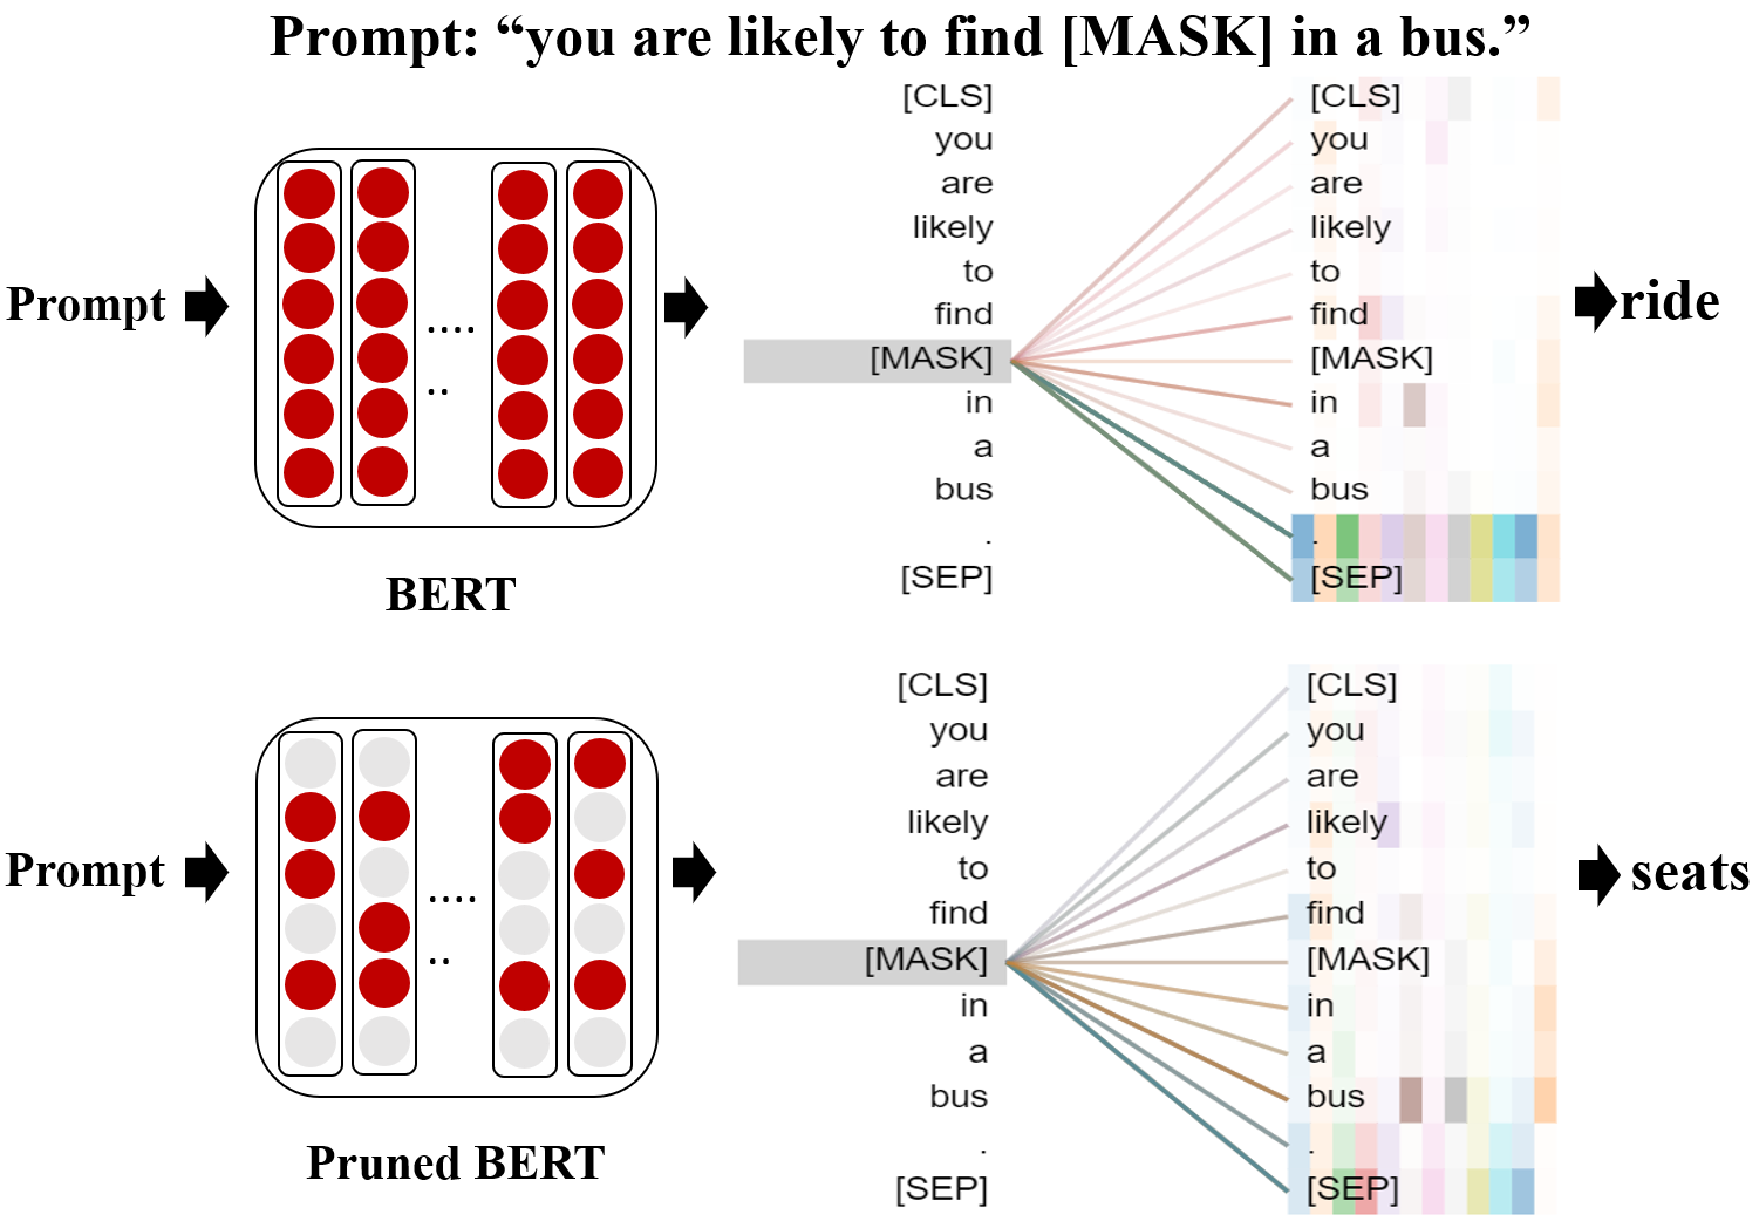
\includegraphics[width=1.0\columnwidth]{figure/intro.pdf}}
	\caption{Querying original/pruned \textsc{BERT-base} with prompts of relation \textit{HasA}. The color spectrum indicates the $12$ attention heads in the last layer~\citep{DBLP:journals/corr/abs-1904-02679}.} \label{fig:LAMA}
\end{figure}


%In summary, our \textbf{contributions} include:
%(i)~We present a novel way of eliciting relational knowledge hidden in PLMs from the perspective of network pruning~(\secref{sec:pruning}). (ii)~Grounding on a concept-centric relation schema, we show that the proposed pruning procedure successfully identified sparse subnetworks specializing in miscellaneous commonsense knowledge remarkably better than their full-scale counterparts~(\secref{sec:LAMA}). (iii)~We showcase the effectiveness of these subnetworks on commonsense knowledge base completion tasks~(\secref{sec:ckbc}) as well as a heuristic application on multiple commonsense reasoning tasks, gleaning insight on the transformation from language representation to knowledge representation.

Code and all pruned subnetworks are open-sourced at \url{https://anonymous.4open.science}.
